\chapter{Annotation Service Documentation}

The following two sections document the implemented functions of the ASS (section \ref{sec_B1}) and ASV (section \ref{sec_B2}) in detail. Both files can be found in the AS' repository at:

 \url{https://github.com/SasNaw/AnnotationService}.

\section{Annotation Service Server}
\label{sec_B1}

\subsubsection{index{\textunderscore}dzi()}
If the client requests a DZI (URL ends in \emph{".dzi"}), \texttt{index{\textunderscore}dzi()} renders an ASV and passes the necessary information (slide URL, file name, MPP) to it.

It builds the file name and slide URL (line 3 and 4) for a requested DZI. A metadata.txt will be present in the [slide name]{\textunderscore}files directory, if the DZI was created with the CS. If so, the function will try to fetch the metadata information about MPP and calculate the average height of a pixel (line 6 - 16). If the MPP metadata could not be fetched, it is set to 0 (line 17 - 18). File name, URL and MPP are then passed onto the ASV, which then is rendered with the given information (line 19).

\begin{lstlisting}[language=Python, frame=single]
@app.route('/wsi/<path:file_path>.dzi')
def index_dzi(file_path):
	file_name = file_path + '.dzi'
	slide_url = '/wsi/' + file_name
	# read dzi file
	try:
		with open('static/wsi/' + file_path + '_files/metadata.txt') as file:
			mpp_x = 0
			mpp_y = 0
			metadata = file.read().split('\n')
			for property in metadata:
				if openslide.PROPERTY_NAME_MPP_X in property:
					mpp_x = property.split(': ')[1]
				elif openslide.PROPERTY_NAME_MPP_Y in property:
					mpp_y = property.split(': ')[1]
			slide_mpp = (float(mpp_x) + float(mpp_y)) / 2
	except IOError:
		slide_mpp = 0
	return render_template('as_viewer.html', slide_url=slide_url, slide_mpp=slide_mpp, file_name=file_name)
\end{lstlisting}


\subsubsection{index{\textunderscore}wsi()}
When the client requests a proprietary WSI (URL \emph{does not} end in ".dzi"), \texttt{index{\textunderscore}wsi()} renders an ASV and passes the necessary information (slide URL, file name, MPP) to it. Furthermore, it wraps a DZG around the proprietary WSI and adds that to the WSGI object.

Line 22 - 27 create a map with the optional DZG parameters (compare tab. \ref{tab4_DZGparam}) and turn them into a dictionary. Line 28 reads the proprietary WSI. A DZG with the supplied parameters\footnote{Compare tab. \ref{tab4_assParams}} is created, which wraps the proprietary slide object to add Deep Zoom support (line 29 - 31). The created DZG is added to the WSGI object (line 29). Line 32 - 37 fetch associated images, the metadata (line 33), wrap the associated images with a DZG of their own and add this, together with the metadata, to the WSGI object. Line 39 - 43 fetch the MPP metadata and calculate the average MPP (or set it to 0, if not found). 
Line 44 creates a URL for the DZG object with Flasks \texttt{url{\textunderscore}for(endpoint, **values)} function. This URL is passed, together with the MPP and file path, to an ASV which then gets rendered (line 45).

\begin{lstlisting}[language=Python, frame=single]
@app.route('/wsi/<path:file_path>')
def index_wsi(file_path):
	config_map = {
		'DEEPZOOM_TILE_SIZE': 'tile_size',
		'DEEPZOOM_OVERLAP': 'overlap',
		'DEEPZOOM_LIMIT_BOUNDS': 'limit_bounds',
	}
	opts = dict((v, app.config[k]) for k, v in config_map.items())
	slide = open_slide('static/wsi/' + file_path)
	app.slides = {
		SLIDE_NAME: DeepZoomGenerator(slide, **opts)
	}
	app.associated_images = []
	app.slide_properties = slide.properties
	for name, image in slide.associated_images.items():
		app.associated_images.append(name)
		slug = slugify(name)
		app.slides[slug] = DeepZoomGenerator(ImageSlide(image), **opts)
	try:
		mpp_x = slide.properties[openslide.PROPERTY_NAME_MPP_X]
		mpp_y = slide.properties[openslide.PROPERTY_NAME_MPP_Y]
		slide_mpp = (float(mpp_x) + float(mpp_y)) / 2
	except (KeyError, ValueError):
		slide_mpp = 0
	slide_url = url_for('dzi', slug=SLIDE_NAME)
	return render_template('as_viewer.html', slide_url=slide_url, slide_mpp=slide_mpp, file_name=file_path)
\end{lstlisting}


\subsubsection{dzi(slug)}
If \texttt{index{\textunderscore}wsi()} was called before, a URL was generated for the WSI. This URL will be requested from the ASS by OpenSeadragon, which causes \texttt{slug(dzi)} to be called. \texttt{slug(dzi)} creates the DZI metadata and returns it to OpenSeadragon.

The \emph{dzi} parameter is the slide URL generated in \texttt{index{\textunderscore}wsi} (line 44).

Line 48 retrieves the format for the individual Deep Zoom tiles. Line 49 - 52 try to create a response. If a response can not be created, because the requested DZG is unknown, a "404 Not Found" http status code will be returned instead. If the DZG could be found, a response with the DZIs metadata will be created via the DZGs \texttt{get{\textunderscore}dzi(format)} function (line 50, compare subsection \ref{sec4_openslide}).

\begin{lstlisting}[language=Python, frame=single]
@app.route('/<slug>.dzi')
def dzi(slug):
	format = app.config['DEEPZOOM_FORMAT']
	try:
		resp = make_response(app.slides[slug].get_dzi(format))
		resp.mimetype = 'application/xml'
		return resp
	except KeyError:
		# Unknown slug
		abort(404)
\end{lstlisting}


\subsubsection{tile(slug, level, col, row, format)}
If a response for OpenSeadragon was created via \texttt{slug(dzi)}, OpenSeadragon will request the individual image tiles in such a way, that, through the use of the route() decorator, \texttt{tile(slug, level, col, row, format)} will be called.

As in \texttt{slug(dzi)}, the \emph{slug} parameter is the slide URL generated in \texttt{index{\textunderscore}wsi} (line 44). The parameters \emph{level}, \emph{col} and \emph{row} describe the DZI level and address of the requested image tile. \emph{format} is the image format of the tile.

If the format is not JPEG or PNG, the ASS return a "404 Not Found" http status code (line 58 - 61).

If the format is either JPEG or PNG, the requested tile is generated through the use of the DZGs \texttt{get{\textunderscore}tile(level, address)} function (line 63). If it was not possible to generate the tile, a "404 Not Found" http status code will be returned.

The generated tile is then saved into a PIL image object\footnote{See \url{http://pillow.readthedocs.io/en/3.3.x/reference/Image.html}}, stored in either a JPEG or PNG image and returned as response to OpenSeadragon (line 70 - 74).

\begin{lstlisting}[language=Python, frame=single]
@app.route('/<slug>_files/<int:level>/<int:col>_<int:row>.<format>')
def tile(slug, level, col, row, format):
	format = format.lower()
	if format != 'jpeg' and format != 'png':
		# Not supported by Deep Zoom
		abort(404)
	try:
		tile = app.slides[slug].get_tile(level, (col, row))
	except KeyError:
		# Unknown slug
		abort(404)
	except ValueError:
		# Invalid level or coordinates
		abort(404)
	buf = PILBytesIO()
	tile.save(buf, format, quality=app.config['DEEPZOOM_TILE_QUALITY'])
	resp = make_response(buf.getvalue())
	resp.mimetype = 'image/%s' % format
	return resp
\end{lstlisting}


\subsubsection{saveJson()}
When the client sends JSON data to save, the \texttt{saveJson()} function is called.

The associated request is a POST request. This means that the posted data needs to be extracted. This can be done via Flasks \emph{request object} (line 77 - 79). The file path will be transmitted as \emph{"source"}, the content to save as \emph{"json"}.

If there is something to save (line 80), the content will be written into the provided file. If the file does not exist yet, it will be created (line 81 - 82).

\begin{lstlisting}[language=Python, frame=single]
@app.route('/saveJson', methods=['POST'])
def saveJson():
	dict = request.form
	source = dict.get('source', default='')
	json = dict.get('json', default='{}').encode('utf-8')
	if len(source) > 0:
		with open('static/' + source, 'w+') as file:
			file.write(json)
	return 'Ok'
\end{lstlisting}


\subsubsection{loadJson()}
When the client requests JSON data, \texttt{loadJson()} is called.

The source of the JSON data is passed in the URL as parameter (\emph{"src=[path to source]"}). The src parameter can be extracted via Flasks request object (line 86). If the provided source is a file, the content will be read and returned as JSON data (line 87 - 90). Otherwise an empty JSON list is returned (line 91 - 92).\clearpage

\begin{lstlisting}[language=Python, frame=single]
@app.route('/loadJson')
def loadJson():
	source = 'static/wsi/' + request.args.get('src', '')
	if os.path.isfile(source):
		with open(source, 'r') as file:
			content = file.read()
			return jsonify(content)
	else:
		return jsonify('[]')
\end{lstlisting}


\subsubsection{createDictionary()}
When the client requests the creation of a new dictionary, \texttt{createDictionary()} is called. The name of the new dictionary is passed as URL parameter (\emph{name= [name]}). The name parameter can be extracted via Flasks request object\footnote{Compare subsection \ref{sec4_flask}} (line 95).

Once the name was extracted, the function checks if a dictionary with the provided name already exists. If so, \emph{"error"} is returned (line 96 - 99). Otherwise a new, empty dictionary is created (line 101 - 102). To switch to the newly created dictionary, the configuration file must be updated (line 103 - 107).

As response, the name and path of the newly created dictionary is returned (line 108 - 109).

\begin{lstlisting}[language=Python, frame=single]
@app.route('/createDictionary')
def createDictionary():
	name = request.args.get('name', '')
	path = 'static/dictionaries/' + name
	if os.path.isfile(path):
		# dictionary already exists
		return 'error'
	else:
		with open(path, 'w+') as dictionary:
			dictionary.write("[]")
		with open('static/configuration.json', 'r') as config:
			content = json.loads(config.read())
			content['dictionary'] = name
		with open('static/configuration.json', 'w+') as config:
			config.write(json.dumps(content))
		respone = '{"name":"' + name + '", "path":"/' + path + '"}'
		return respone
\end{lstlisting}


\subsubsection{getDictionaries()}
The \texttt{getDictionaries()} function is called, when the client requests a list of all available dictionaries.

If no dictionaries could be found, "-1" will be returned, otherwise a JSON list of all available dictionaries.

\begin{lstlisting}[language=Python, frame=single]
@app.route('/getDictionaries')
def getDictionaries():
	dir = 'static/dictionaries/'
	if os.path.isfile(dir):
		# no dictionaries found
		return '-1'
	else:
		# return dictionaries
		return json.dumps(os.listdir(dir))
\end{lstlisting}


\subsubsection{runSegmentation()}
The \texttt{runSegmentation()} function is called, when the client tags a POI. It imports the python script provided in the configuration file\footnote{
	Compare tab. \ref{tab4_assConfig} in subsection \ref{sec4_setup}.
} as module and calls the module's \texttt{run(x,y)} function.

The function uses Flasks \emph{request object} to acquire the provided x and y coordinates from the provided URL (line 3 \& 4). It then opens the configuration file and extracts the name of the segmentation script (line 5 - 7). If no name was provided for the script (string is empty) the server will print an error message and return with a "404 Not Found" HTTP status code (line 8 - 11).

If a script name was provided and successfully extracted, it is imported as python module (line 13, 14). If the import was successful, the script's run method is called and the returned contour will be passed back to the server as JSON data (line 15 - 16).

If the script could not be imported, a error message will be printed by the server and a "404 Not Found" HTTP status code is returned (line 18 - 20).

\begin{lstlisting}[language=Python, frame=single]
@app.route("/runSegmentation")
def runSegmentation():
	x = request.args.get('x', '0')
	y = request.args.get('y', '0')
	with open("static/configuration.json", 'r') as file:
		config = json.loads(file.read())
		module_name = config.get("segmentationScript")
	if(len(module_name) == 0):
		print("ERROR: no segmentation script provided 
				in configuration file (configuration.json)!")
		return "404"
	try:
		module = __import__("static.segmentation.%s" % (module_name),
				fromlist=["segmentation"])
		contour = module.run(x,y)
		return json.dumps(contour)
	except ImportError:
		print("ERROR: provided segmentation script (" + module_name +
				") not found!")
		return "404"
\end{lstlisting}


\section{Annotation Service Viewer}
\label{sec_B2}

Since the ASV has \textgreater 2,000 lines of code, there will be no documentation of every single line of code\footnote{
	The implementation of the ASV can be found in its GIT repository at: \url{https://github.com/SasNaw/AnnotationService}
}. Instead a description of every function is provided. Code snippets are present, when necessary or helpful for understanding.


\subsection{Initialization functions}

\subsubsection{function init(file{\textunderscore}name, url, mpp)}
\emph{Parameters:\\
	file{\textunderscore}name: name of the requested WSI\\
	url: URL to the DZI's metadata file\\
	mpp: microns per pixel of the requested WSI\\ \\
}
The \texttt{init(file{\textunderscore}name, url, mpp)} is called by the \emph{as{\textunderscore}viewer.html} to start the initialization of the ASV JavaScript. The parameters are served by the ASS. \emph{file{\textunderscore}name} describes the name of the WSI, \emph{url} contains the URL to the DZI metadata file and \emph{mpp} equals the microns per pixel of the requested WSI (if that information could be retrieved from the metadata, 0 otherwise).

The function requests the content of the configuration file (via \texttt{loadConfiguration()}) from the ASS and creates the OSDV (via \texttt{initAnnotationService()}, see fig. \ref{figB_init}).

\begin{figure}[H]
	\begin{center}
		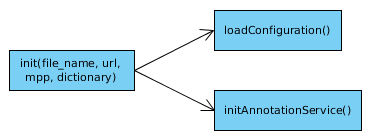
\includegraphics[scale=0.5]{img/ch_init.png}
		\caption{Call hierarchy of \texttt{init(file{\textunderscore}name, url, mpp)}}
		\label{figB_init}
	\end{center}
\end{figure}


\subsubsection{function initAnnotationService()}
\texttt{initAnnotationService()} selects the navigation tool (via \texttt{selectTool()}), creates the OSDV and its scalebar. It then opens the tile source at the URL specified in the \texttt{init(file{\textunderscore}path, url, mpp)} function. Additionally, event handlers to are set up to react to:
\begin{itemize}
	\item mouse interaction
	\item opening of a WSI
	\item zooming
\end{itemize}
Furthermore, the toolbar is initialized.

Once a tile source was opened, the AO is initialized (via \texttt{initAnnotationOverlay()}) and the saved annotations are requested (via \texttt{loadJson()}, see fig. \ref{figB_initAS}).

\begin{figure}[H]
	\begin{center}
		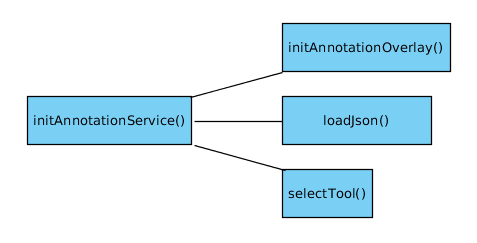
\includegraphics[scale=0.5]{img/ch_initAS.png}
		\caption{Call hierarchy of \texttt{initAnnotationService()}}
		\label{figB_initAS}
	\end{center}
\end{figure}


\subsubsection{function initAnnotationOverlay()}
\texttt{initAnnotationOverlay()} creates the ASV's AO. The AO is transformed to the size of the OSDV via the \texttt{transform()} function.


\subsection{Data management functions}

\subsubsection{function loadConfiguration()}
\texttt{loadConfiguration()} requests and parses the content of the configuration file from the ASS. Furthermore, it requests the list of available dictionaries (via \texttt{getDictionaryList()}) and loads the content of the dictionary specified in the configuration (via \texttt{loadDictionary(path)}, see fig. \ref{figB_loadConfig}).

\begin{figure}[H]
	\begin{center}
		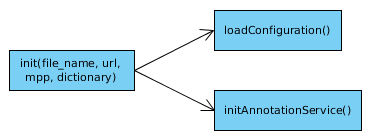
\includegraphics[scale=0.5]{img/ch_init.png}
		\caption{Call hierarchy of \texttt{loadConfiguration()}}
		\label{figB_loadConfig}
	\end{center}
\end{figure}


\subsubsection{function getDictionaryList()}
\texttt{getDictionaryList()} requests a list of all dictionaries from the ASS. The received list is then added as a clickable list to the toolbar.


\subsubsection{function loadDictionary(path)}
\emph{Parameters:\\
	path: file path of the requested dictionary\\ \\
}
\texttt{loadDictionary(path)} requests the content of the dictionary file at \emph{path} from the ASS. The response is either a list of entries, which are then added to the list of available labels in the toolbar (via \texttt{appendLabelsToList()}), or a -1, if no dictionary was found. In this case, the ASV forces the user to create a new, empty dictionary (via \texttt{createNewDictionary(isCancelable)}, see fig. \ref{figB_loadDict}).

\begin{figure}[H]
	\begin{center}
		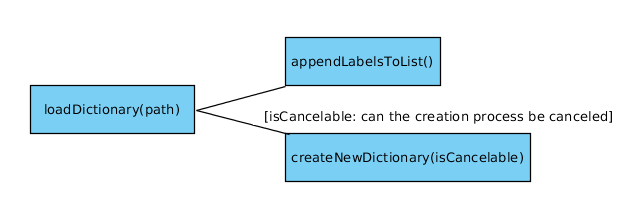
\includegraphics[scale=0.5]{img/ch_loadDict.png}
		\caption{Call hierarchy of \texttt{loadDictionary(path)}}
		\label{figB_loadDict}
	\end{center}
\end{figure}


\subsubsection{function loadJson()}
\texttt{loadJson()} requests the saved annotations for the provided WSI. If an annotation file could be loaded by the ASS, a list of region data is returned. Each entry of the region data list is then turned into an actual region and added to the region list (via \texttt{newRegion(arg, imageNumber)}, see fig. \ref{figB_loadJson}).

\begin{figure}[H]
	\begin{center}
		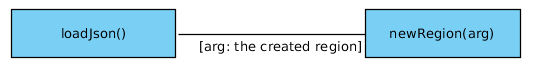
\includegraphics[scale=0.5]{img/ch_loadJson.png}
		\caption{Call hierarchy of \texttt{loadJson()}}
		\label{figB_loadJson}
	\end{center}
\end{figure}


\subsubsection{function createNewDictionary(isCancelable)}
\emph{Parameters:\\
	isCancelable: 1 if the process can be canceled without providing a valid dictionary name, 0 otherwise\\ \\
}
\texttt{createNewDictionary(isCancelable)} opens a prompt and asks the user to provide a name for the dictionary to create. If \emph{isCancelable} is true (1), the prompt can be closed and the creation process is canceled. If it is false (0), the prompt will be shown until a valid name was provided.

After creation of the new dictionary it is selected as active one (and its empty content is loaded via \texttt{loadDictionary(path)}) and the list of available dictionaries is updated (via \texttt{getDictionaryList()}, see fig. \ref{figB_createDict}).

\begin{figure}[H]
	\begin{center}
		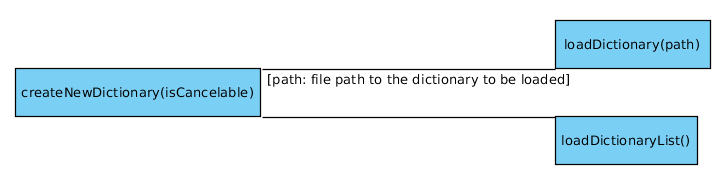
\includegraphics[scale=0.45]{img/ch_createDict.png}
		\caption{Call hierarchy of \texttt{createNewDictionary(isCancelable)}}
		\label{figB_createDict}
	\end{center}
\end{figure}


\subsection{GUI functions}

\subsubsection{function selectTool()}
\texttt{selectTool()} changes the mouse cursor to the icon of the currently selected tool.


\subsubsection{function transform()}
\subsubsection{function appendLabelsToList()}
\subsubsection{function appendLabelToList(label)}



\subsection{Region functions}
\subsubsection{function newRegion(arg, imageNumber)}


%-----------------------------------------------------------------------
\subsubsection{function newLabel()}

\subsubsection{function selectNextLabel()}
\subsubsection{function selectLabel(el)}

\subsubsection{function findContextRegion(region1)}
\subsubsection{function isRegionAlreadyReferenced(region1, region2)}
\subsubsection{function removeRegion(reg, imageNumber)}
\subsubsection{function selectRegion(reg)}
\subsubsection{function deselectRegion(reg)}
\subsubsection{function findRegionByUID(uid)}
\subsubsection{function findRegionByName(name)}
\subsubsection{function hash(str)}
\subsubsection{function regionHashColor(name)}
\subsubsection{function regionPicker(parent)}
\subsubsection{function changeRegionName(reg,name)}
\subsubsection{function toggleAllRegions()}
\subsubsection{function toggleRegions(uid)}
\subsubsection{function changeRegionAnnotationStyle(uid)}
\subsubsection{function convertPathToImgCoordinates(point)}
\subsubsection{function convertImgToPathCoordinates(point)}
\subsubsection{function clickHandler(event)}
\subsubsection{function addPoi(event}
\subsubsection{function pressHandler(event)}
\subsubsection{function dragHandler(event)}
\subsubsection{function singleClickOnLabel(event)}
\subsubsection{function singlePressOnRegion(event)}
\subsubsection{function doublePressOnRegion(event)}
\subsubsection{function mouseDown(x,y)}
\subsubsection{function mouseDrag(x,y,dx,dy)}
\subsubsection{function getDistance()}
\subsubsection{function mouseUp()}
\subsubsection{function pad(number, length)}
\subsubsection{function annotationStyle(label)}
\subsubsection{function setRegionColor()}
\subsubsection{function onFillColorPicker(value)}
\subsubsection{function onAlphaSlider(value)}
\subsubsection{function onAlphaInput(value)}
\subsubsection{function cmdUndo()}
\subsubsection{function cmdRedo()}
\subsubsection{function getUndo()}
\subsubsection{function saveUndo(undoInfo)}
\subsubsection{function setImage(imageNumber)}
\subsubsection{function applyUndo(undo)}
\subsubsection{function commitMouseUndo()}
\subsubsection{function finishDrawingPolygon(closed)}
\subsubsection{function backToPreviousTool(prevTool)}
\subsubsection{function backToSelect()}
\subsubsection{function cmdDeleteSelected()}
\subsubsection{function clearToolSelection()}
\subsubsection{function toolSelection(event)}

\subsubsection{function saveJson(json, filePath)}
\subsubsection{function saveConfig()}
\subsubsection{function saveDictionary()}
\subsubsection{function getJsonSource()}
\subsubsection{function saveRegions()}

\subsubsection{function loadImage(name)}
\subsubsection{function resizeAnnotationOverlay()}


\subsubsection{function toggleDictPicker()}
\subsubsection{function dictListClick(index)}


\subsubsection{function initAnnotationService()}
\subsubsection{function help(show)}
\subsubsection{function toggleMenu ()}
\subsubsection{\$(document).keydown(function(e)}
\subsubsection{function selectToolOnKeyPress(id)}

\subsubsection{\$(document).keyup(function(e)}
